\documentclass[cn,10pt,math=newtx,chinesefont=founder]{elegantbook}
\usepackage{graphicx}
\title{物理中的數學}
\subtitle{2021年}

\author{李宥頡、王琳嘉}
\institute{拓普科學組}
%\date{May 2, 2021}
%\version{4.1}
%\bioinfo{自定义}{信息}

%\extrainfo{寶寶肚子餓—— 顏利蓁}

\setcounter{tocdepth}{3}

%\logo{logo-blue.png}
\cover{cover.jpg}

% 本文档命令
\usepackage{array}
\newcommand{\ccr}[1]{\makecell{{\color{#1}\rule{1cm}{1cm}}}}

\definecolor{customcolor}{RGB}{32,178,170}
\colorlet{coverlinecolor}{customcolor}

\begin{document}

\maketitle
\frontmatter

\tableofcontents

\mainmatter

\chapter{三角函數}
\section{意義}
    三角函數描述角度與邊長比值的函數關係,由相似形可以知道,固定角度的三角形,其邊長之間的比例也為固定。故我們只要知道三角形的
    一邊和一角,即可表示其他邊。換句話說,三角函數就是由角度(自變數)得到邊長比例(應變數)。
\section{銳角三角函數}
定義一個直角三角形,並使角度為$\theta$,規定直角三角形的三邊分別為


\begin{minipage}{\linewidth}
      \begin{minipage}{0.45\linewidth}
\raggedleft
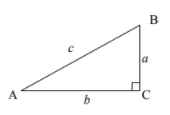
\includegraphics[scale=1]{image/直角三角形.png}
      \end{minipage}
      \hspace{0.05\linewidth}
      \begin{minipage}{0.45\linewidth}
\raggedright
\begin{enumerate}
    \item 斜邊c(最長邊)
    \item 對邊b(正對$\theta$)
    \item 鄰邊a(和$\theta$相鄰)
\end{enumerate}
      \end{minipage}
\end{minipage}

一般來說有六個三角函數
\begin{enumerate}
    \itemsep= 10pt
    \item 正弦$\sin \theta = \frac{a}{c}$
    \item 餘弦$\cos \theta = \frac{b}{c}$    
    \item 正切$\tan \theta = \frac{a}{b}$    
    \item 正割$\sec \theta = \frac{c}{b}$
    \item 餘割$\csc \theta = \frac{c}{a}$
    \item 餘切$\cot \theta = \frac{b}{a}$
\end{enumerate}

\section{命名的由來}
\begin{figure}
    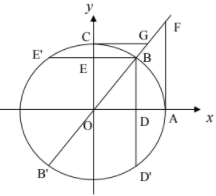
\includegraphics[width=0.3\textwidth]{image/單位圓2.png}

\end{figure}
\newpage

\section{特殊角}
    物理常見的特殊角度有 30、37、45、53、60,從直
    角三角形的邊長比值可求出它們的三角函數。
\begin{figure}[h]
    \flushleft
    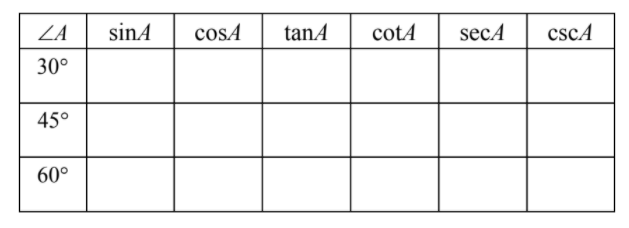
\includegraphics[width=0.5\textwidth]{image/special.png}
\end{figure}

\section{基本關係}
\begin{enumerate}
    \item 倒數關係
    \begin{itemize}
        \item $\sin \theta \csc \theta = 1$
        \item $\cos \theta \sec \theta = 1$
        \item $\tan \theta \cot \theta = 1$
    \end{itemize}
    \item 平方關係
    \begin{itemize}
        \item $\sin^2 \theta + \cos^2 \theta = 1 $        
        \item $ 1 + \tan^2 \theta = \sec^2 \theta$
        \item $ 1 + \cot^2 \theta = \csc^2 \theta $
    \end{itemize}
    \item 商數關係
    \begin{itemize}
        \itemsep = 8pt
        \item $\frac{\sin \theta}{\cos \theta}= \tan \theta$
        \item $\frac{\cos \theta}{\sin \theta}= \cot \theta$
    \end{itemize}
    \item 互餘關係
    \begin{itemize}
        \item $\sin (90^\circ - \theta) = \cos \theta$, $\cos (90^\circ - \theta) = \sin \theta$
        \item $\tan (90^\circ - \theta) = \cot \theta$, $\cot (90^\circ - \theta) = \tan \theta$
        \item $\sec (90^\circ - \theta) = \csc \theta$, $\csc (90^\circ - \theta) = \sec \theta$
    \end{itemize}


\end{enumerate}

\section{補充}
\newpage

\section{應用}
由於物理上經常將向量(有大小有方向的量)依照兩個正交的方向分解,
因此配合三角函數,就可以輕鬆表示分量。且由於運動獨立性,互相正交的運動不會互相干擾,方便計算。
\begin{enumerate}
    \itemsep = 20em
    \item 斜面
    \item 斜拋
    \item 三力平衡
\end{enumerate}
\newpage

\chapter{微積分}
\section{斜率}
 斜率是用來表示一直線的傾斜程度,亦即橫坐標向正方向
 每前進一格,縱坐標上升或下降多少格。物理上,橫軸常為時間,則斜率表示物理量的時變率。
\begin{equation}
    slope =  m  = \tan \theta = \frac{\Delta y}{\Delta x}
\end{equation}
若函數圖形並非直線,而是曲線,則斜率需區分為割線斜率與切線斜率。
\begin{enumerate}
    \itemsep = 2em
    \item 割線斜率=平均時變率=一段時間內某物理量的變化率=$\frac{\Delta y}{\Delta x}$
    \item 切線斜率=瞬間時變率=某個時刻上某物理量的變化率=$\frac{dy}{dx}$ = 微分
\end{enumerate}
\section{函數下的面積}
 函數圖形下的面積代表累積量,物理上橫軸常為時間,則函數下的面積代表物理量隨時間的累積量。
 若函數為直線,則面積大多可以利用基礎幾何求出,不過若函數為曲線,則面積須以積分求出。
\section{多項式微積分}
多項式(polynoimal)代表函數的每一項都可以表示為$cx^n$,在中學範疇比較常用,故在此介紹。
\begin{enumerate}
    \item 指數向前乘係數
    \item 次方降一次
    \item 常數微分為零
\end{enumerate}
由微積分基本定理,可知微分積分互為逆運算,由上面規則即可反推出積分規則。\\
練習:
\newpage
\section{補充}
\newpage
\end{document}

